% 导言区
\documentclass[UTF-8]{article} %article

\usepackage{ctex} 					% 用于支持中文输入
\usepackage{graphicx}			 % 用于支持插入图片
\usepackage{bm}						% 用于加粗公式,\textbf{text} 是用于加粗普通文本,不能用于加粗公式
\usepackage{color}					% 文字增加颜色

\title{深度学习}
\author{周康}
\date{\today}

%\graphicspath{pictures/逻辑回归/}


%正文区
\begin{document}
	\maketitle
	\tableofcontents
	
	\section{神经网络相关概念}
	\subsection{逻辑回归函数-线性预测结果}
	\textbf{逻辑回归函数作用:线性预测结果。}
	\begin{equation}
		\bm{z = dot(w, x) + b} \label{eq:logistic1}
	\end{equation}
	
	
	其中,$x$是特征向量,以图像大小$64 \times 64$个像素为例,每个像素由红绿蓝$RGB$三个颜色组成,那么图像向量的维度为64 $\times$ 64 $\times$ 3 = 12288,在人工智能领域,每一个输入到神经网络的数据都叫做一个特征,所以这张图就有12288个特征,一般我们转化为一维向量1 $\times$ 12288(行向量),或者12288 $\times$ 1(列向量)来进行计算。
	
	$w$是$x$的权重,代表了每个特征的重要程度,b是阈值,用来影响预测结果,z就是预测结果。公式中的$dot()$函数表示将w和x进行向量相乘。
	
	为简便起见,假定$x$为行向量,有3个特征,即$x=(x_1, x_2, x_3)$,相应的$w$为列向量,也有3个权重分量,即$w=(w_1, w_2, w_3)^T$,此时公式\ref{eq:logistic1}可以转化为:

	\begin{equation}
		\bm{z = w_1 \cdot x_1 + w_2 \cdot x_2 + w_3 \cdot x_3 + b} \label{eq:logistic2}
	\end{equation}
	假定这是用来预测图片是否为猫,$z>0$表示有猫,$z<=0$表示无猫,当预测结果$z=10$时,表示图片有猫。
	
	公式\ref{eq:logistic2}可以用图\ref{fig:1nn}所示。
	
	\begin{figure}[htb]			% figure 浮动图片,htb选项用的最多
		\centering
		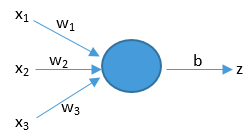
\includegraphics[width=8cm, height=3cm]{pictures/逻辑回归/1nn}
		\caption{逻辑回归}
		\label{fig:1nn}
	\end{figure}

	\subsection{激活函数-非线性预测结果}
	\textbf{激活函数作用:预测结果,非线性,既有突变性,类似于神将元的突触,真正提高神经网络智商的函数。}
	
	在实际的神经网络中,我们不能直接使用逻辑回归,必须在逻辑回归外面加一个激活函数,如果没有它,神经网络永远智商高不起来,激活函数种类很多,这里介绍sigmoid函数。
	\begin{equation}
		\bm{y' = \sigma (Z) = \frac{1}{1 + e^{-Z}}} \label{eq:sigmoid}
	\end{equation}
	公式\ref{eq:sigmoid}对应的图像如图\ref{fig:sigmoid}所示。

	\begin{figure}[htb]
		\centering
		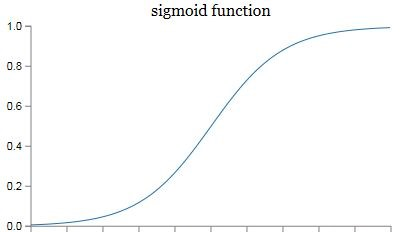
\includegraphics[width=0.7\linewidth]{pictures/激活函数/sigmoid}
		\caption{激活函数}
		\label{fig:sigmoid}
	\end{figure}

	sigmoid函数的一个作用就是把$z$映射到$[0, 1]$之间,上图的横坐标是$z$,纵坐标用$y'$表示,$y'$就代表了最终的预测结果,从图像中可以看出,$z$越大,$y'$就越靠近1,$z$越小,$y'$就越靠近0,把预测结果映射到$[0, 1]$,有利于神经网络的计算,也便于人类进行理解,在预测猫的例子中,如果$y'$是0.8,就说明有80\%的概率是猫。

	\subsection{损失函数-预测与实际的差距}
	\textbf{损失函数作用:判断单个训练样本的预测结果与实际结果的差距}
	
	先回顾一下先前的预测算法,如下:	
	$$\bm{\hat{y}^{(i)} = \sigma (w^Tx^{(i)}) + b}$$
	$$\bm{\sigma (Z^{(i)}) = \frac{1}{1 + e^{-Z^{(i)}}}}$$
	
	其中$\hat{y}$是预测结果,角标$i$指代第$i$个训练样本,$\hat{y}^{(i)}$是对于训练样本$x^{(i)}$的预测结果。
	$$\bm{L(\hat{y}^{(i)}, y^{(i)}) = \frac{1}{2}(\hat{y}^{(i)} - y^{(i)})^2}$$
	
	损失函数运算后的结果越大,那么预测就与实际结果的偏差越大,即预测精度越低。理论上可以用上面的公式作为损失函数--预测结果与实际结果的差的平方再乘以二分之一。但是在实践中通常不使用它,而是使用公式\ref{eq:loss_function}:
	\begin{equation}
		\bm{L(\hat{y}^{(i)}, y^{(i)}) = -(y^{(i)}log(\hat{y}^{(i)}) + (1 - y^{(i)})log(1 - \hat{y}^{(i)}))} \label{eq:loss_function}
	\end{equation}
	
	这个新的损失函数作用与之前相同,努力使损失函数的值越小,就是努力让预测的结果越准确。
	
	\subsection{成本函数-预测与实际的差距}
	\textbf{成本函数作用:判断整个训练集的预测结果与实际结果的差距}
	
	损失函数是针对单个训练样本来定义的,成本函数是用来衡量整个训练集的预测精度。其实就是对每个训练样本的“损失”进行累加,然后求平均值。成本函数的公式如下:
	\begin{equation}
		\bm{J(w,b) = \frac{1}{m}\sum_{i=1}^{m}L(\hat{y}^{(i)}, y^{(i)}) = - \frac{1}{m}\sum_{i=1}^{m}[(y^{(i)}log(\hat{y}^{(i)}) + (1 - y^{(i)})log(1 - \hat{y}^{(i)}))]} \label{eq:cost}
	\end{equation}

	损失函数定义:将随机事件或有关随机变量的取值映射为非负实数以表示该随机事件的风险或损失的函数。
	
	损失函数的作用就是衡量模型预测的好坏,换一种说法就是衡量两个分布之间的距离:其中一个分布是原始分布,或者正确的分布,而另一个分布则是目前的分布,或者模型拟合的分布。
	
	\subsection{梯度下降法-神经网络的学习功能}
	\textbf{梯度下降法作用:预测是否准确由成本函数确定,而成本函数由权重w和阈值b影响,梯度下降法就是为了找出合适的w和b,一步步的调整w和b,新的w和b会使成本函数的输出结果更小,进一步让预测结果更加准确。}

	回顾逻辑回归算法和损失函数,结合下面几个公式,输入x和实际结果y都是固定的,所以损失函数是一个关于w和b的函数,所谓“学习”或“训练神经网络”,就是找到一组w和b,使损失函数最小。
	$$\bm{\hat{y}^{(i)} = \sigma (w^Tx^{(i)}) + b}$$
	$$\bm{\sigma (Z^{(i)}) = \frac{1}{1 + e^{-Z^{(i)}}}}$$
	$$
		\bm{J(w,b) = \frac{1}{m}\sum_{i=1}^{m}L(\hat{y}^{(i)}, y^{(i)}) = - \frac{1}{m}\sum_{i=1}^{m}[(y^{(i)}log(\hat{y}^{(i)}) + (1 - y^{(i)})log(1 - \hat{y}^{(i)}))]}
	$$
	
	\begin{figure}[htb]
		\centering
		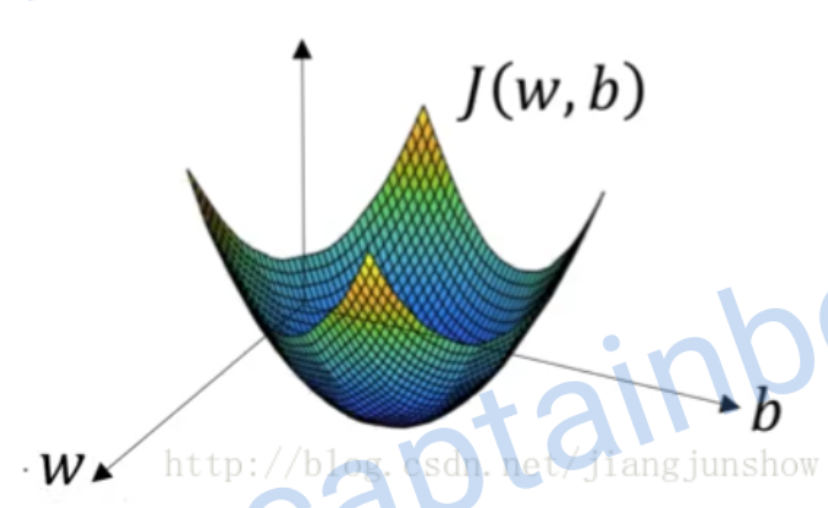
\includegraphics[width=0.7\linewidth]{pictures/成本/lost}
		\caption{成本函数}
		\label{fig:lost}
	\end{figure}

	如图\ref{fig:lost}所示,损失函数$J$的形状是一个漏斗状,我们训练的目标就是找到漏斗底部的一组$w$和$b$,这种漏斗状的函数被称为凸函数(这里指的是向下凸),我们选择公式\ref{eq:loss_function}作为损失函数的真正原因正是因为它是一个凸函数。

	\begin{figure}[htb]
		\centering
		
\includegraphics[width=0.7\linewidth]{pictures/梯度下降法/gradient_descent1}
		\caption{}
		\label{fig:gradient_descent1}
	\end{figure}
	
	如图\ref{fig:gradient_descent1}所示,梯度下降法会一步步地更新$w$和$b$,使损失函数一步步地变小,最终找到最小值或接近最小值的地方。
	\begin{figure}[htb]
		\centering
		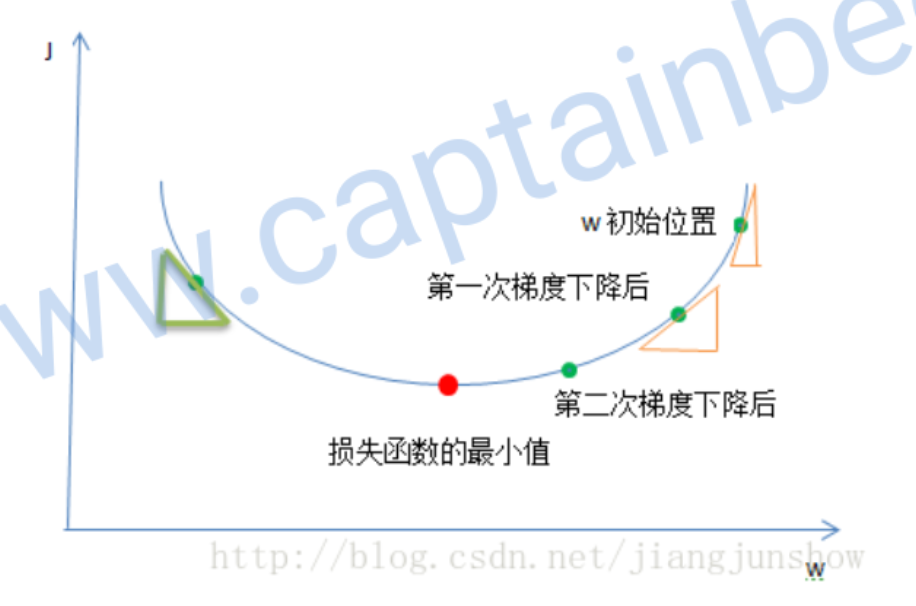
\includegraphics[width=0.7\linewidth]{pictures/梯度下降法/gradient_descent2}
		\caption{}
		\label{fig:gradient_descent2}
	\end{figure}
	
	为了简化问题,先假设损失函数$J$只有一个参数$w$,并且假设$w$只是一个实数(实际上$w$是一个向量)。如图\ref{fig:gradient_descent2}所示,梯度下降算法一步步改变着$w$的值,使损失函数的结果越来越小。
	\begin{equation}
		\bm{w' = w - r * \frac{dJ}{dw}} \label{eq:gradient_descent}
	\end{equation}
	这里的$\frac{dJ}{dw}$就是图\ref{fig:gradient_descent2}中的斜率,这里的$w'$是下一次$w$的值(注意,这里$w'$不是导数),假定$\Delta w = w - w'$,那么\ref{eq:gradient_descent}可以转化为$\Delta w = r * \frac{dJ}{dw}$。所以这里的\textcolor{red}{\textbf{$r$可以理解成$\Delta J$,所以学习率$r$就是成本函数$J$的$dJ$}}。
	
	为简化起见,在床长人工智能教程中,$\textcolor{red}{\textbf{$\frac{dJ}{dw}$}}$省略写成$\textcolor{red}{\textbf{dw}}$,所以,公式\ref{eq:gradient_descent}可以写成如下形式:
	\begin{equation}
		\textcolor{red}{\bm{w' = w - r * dw} \label{eq:gradient_descent2}}
	\end{equation}

	\subsubsection{解释与说明}
	在梯度下降法中,有几点需要重点解释与说明一下:
	\begin{itemize}
		\item 损失函数为什么不选择平方差乘以$\frac{1}{2}$,而是采用\ref{eq:loss_function}的形式?
	\end{itemize}



\end{document}